Using the result of the first derivative equal to zero, we can plug in any pair $k_1, k_2$ and use the inverse CDF of the histogram for the given data to determine the estimator that minimizes the expected loss. That is to say the following:
\begin{align*}
    \hat{u} = F_\theta^{-1}\left(\frac{k_2}{k_1+k_2}\right)
\end{align*}

Thus, with $(k_1, k_2) = (20, 40)$, we determine an estimator $\mathbf{\hat{u}=20.56}$ for 50 bins in the CDF:
\begin{center}
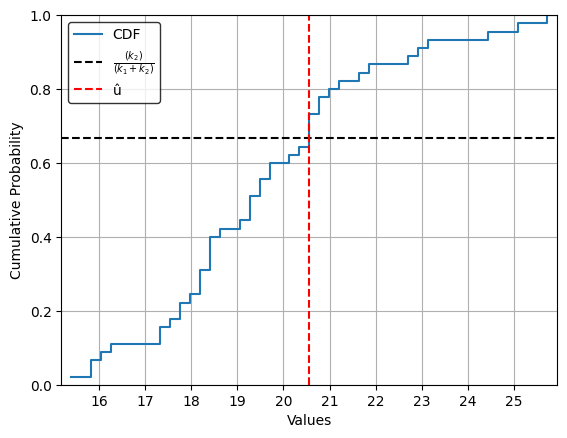
\includegraphics[scale=0.8]{data/05_reporting/problem_set_2/pset2p2.5.1.png}
\end{center}

Next, with $(k_1, k_2) = (0.5, 6)$, we determine an estimator $\mathbf{\hat{u}=23.14}$ for 50 bins in the CDF:
\begin{center}
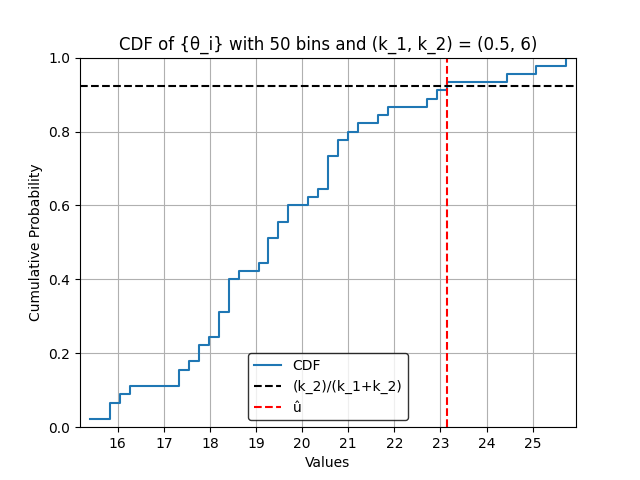
\includegraphics[scale=0.8]{data/05_reporting/problem_set_2/pset2p2.5.2.png}
\end{center}
